\hypertarget{drive-systems}{%
\section{Drive Systems}\label{drive-systems}}

There are as many different drives systems as ways to mount wheels on
frames. Well, almost. What we will do here is to cover a few common
designs and leave the more exotic systems to the mechanical engineering
literature. Vehicle design is fun and we could devote many pages to the
subject. However, in practice we really only see a limited number of
drive systems and those are the one we will discuss. So, we get started
with a simple system, the bicycle, which we will use to introduce some
basic concepts. Then we present the equations of motion for the
differential drive, omniwheel designs and the front wheel steered
designs. The derivations for these systems are presented in the
Kinematics chapter later on.

\hypertarget{basic-constraints-and-the-icr}{%
\subsection{Basic constraints and the
ICR}\label{basic-constraints-and-the-icr}}

We will assume two basic contraints about our wheels. The first is
\emph{no slip} which will mean that the wheel has perfect traction and
the distance around the wheel translates into the same linear distance.
This condition is broken when we lose traction on surfaces with ice,
snow or mud. The next constraint is the \emph{no slide} constraint. This
constraint means that we always move in the direction the wheel is
pointed and not in the axle direction. This constraint can be violated
on slick surfaces where the rotational motion of the craft causes the
vehicle to slide sideways, again on ice, snow or mud. There are a couple
of common vehicle designs that explicitly violate one or both conditions
in order to turn. Examples include tank or treaded systems and skid
steer systems like Bobcats. Many hobby robots have four driven but not
steered wheels which are skid steer. This is not a bad thing, just that
we cannot use the kinematic equations based on the no slip / no slide to
model steered motion. In practice this is not a significant problem.

\begin{figure}
\centering
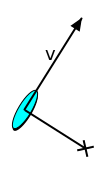
\includegraphics[width=0.15\textwidth,height=\textheight]{MotionFigures/ICR0.*}
\caption{No slide condition means the wheel motion is in the direction
of v. No slip means the distance traveled is the same as the wheel arc
distance traveled.}
\end{figure}

The no-slide assumption means that there is no motion in the direction
of the axle. All of the motion is perpendicular to the axle. This means
for each wheel, the no slide constraint generates a zero motion line
orthogonal to the wheel plane.

The intersection of the zero motion lines is the ICR - Instantaneous
Center of Rotation. Having a common intersection, an ICR, implies that
each wheel is moving on a concentric circle. If the zero motion lines do
not intersect at a single point, then no motion is possible when we have
no-slip and no-slide for our wheels. We can easily see that this is the
case for the simple steering approach shown above. The rear wheels have
overlapping zero motion lines. The front wheels have parallel
non-overlapping zero motion lines. All intersect at the ICR. Note that
parallel lines intersect at infinity so we don't have to have a finite
intesection.

\begin{figure}
\centering
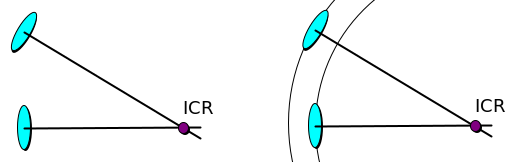
\includegraphics[width=0.7\textwidth,height=\textheight]{MotionFigures/ICR1.*}
\caption{ICR - Instantaneous Center of Rotation.}
\end{figure}

\hypertarget{differential-drive}{%
\subsection{Differential Drive}\label{differential-drive}}

One of the most common drive system in robotics is the differential
drive. Differential drive is a two wheeled drive system. For stability a
third support must be employed. A castor wheel or ball is normally used.
The well known Rumba floor cleaning robot uses this system. It is
stable, maneuverable, easy to control, and simple. \texttt{ddrive\_pre}
gives the basic layout and variables involved in the model.

\begin{quote}
The differential drive robot dimensions and variables.
\end{quote}

Recall the Differential Drive robot setup~\texttt{fig:ddriveRecalled2}:

\begin{quote}
Simple differential drive robot.
\end{quote}

and the forward kinematics:

\[\begin{aligned}
\boxed{
\begin{array}{l}
 \dot{x} = \frac{r}{2} (\dot{\phi_1}+\dot{\phi_2})\cos(\theta) \\[5mm]
\dot{y} = \frac{r}{2} (\dot{\phi_1}+\dot{\phi_2})\sin(\theta) \\[5mm]
\dot{\theta} = \frac{r}{2L} (\dot{\phi_1}-\dot{\phi_2})
\end{array}}
\end{aligned}\]

and the inverse kinematics:

\[\begin{aligned}
\boxed{
\begin{array}{l}
v = \sqrt{\dot{x}^2 + \dot{y}^2},\\[2mm]
\kappa =   \displaystyle  \frac{\dot{x}\ddot{y} - \dot{y}\ddot{x}}{v^3} \\[3mm]
\dot{\phi_1} = \displaystyle \frac{v}{r}\left(\kappa L + 1\right) \\[3mm]
\dot{\phi_2} = \displaystyle \frac{v}{r}\left(-\kappa L + 1\right)
\end{array}}
\end{aligned}\]

where \(\dot{\phi_1}\) and \(\dot{\phi_2}\) be the right and left wheel
rotational speeds (respectively), \(r\) is wheel radius and \(L\) is the
axle length from the center to the wheel (``half axle'').

\hypertarget{alternate-form}{%
\subsubsection{Alternate Form}\label{alternate-form}}

In some cases we only need to know the forward velocity and the vehicle
rotation rate. By computing \(v\) from \texttt{ddkinematicsmodel} and
using \(\omega = \dot{\theta}\), we obtain

\[\begin{aligned}
\begin{array}{l}
v = \frac{r}{2} (\dot{\phi_1}+\dot{\phi_2}) \\[5mm]
\omega = \frac{r}{2L} (\dot{\phi_1}-\dot{\phi_2})
\end{array}
\end{aligned}\]

and the inverse of these are

\[\begin{aligned}
\begin{array}{l}
\dot{\phi_1} = \frac{1}{r} (v+L\omega)\\[5mm]
\dot{\phi_2} = \frac{1}{r} (v-L\omega)
\end{array}
\end{aligned}\]

\hypertarget{omniwheels}{%
\subsection{Omniwheels}\label{omniwheels}}

\texttt{gammaconfig} shows some sample types of omniwheels using the
\(\gamma = 0\) configuration and \(\gamma = 45^\circ\) configuration.
Also recall that \(\gamma=0\) style of wheel is used in non-parallel
mounting as shown in the first robot in the \texttt{gammawheelmounting}
and the parallel mounting is used for the other standard type of wheel
design using \(\gamma = 45^\circ\).

\begin{quote}
Dimensions for the Mecanum Kinematics.
\end{quote}

For this section we assume that we have a traditional care design frame
and wheel mounting as described in \texttt{fig:mecanumdim}
(\(\gamma = 45^\circ\)). The following notation is used in the
kinematics:

\begin{itemize}
\tightlist
\item
  \(r\) - wheel radius.
\item
  \(L_1\) - half-distance between left and right wheel pairs, \(L_2\) -
  half-distance between front and rear wheel pairs.
\item
  \(v_x\), \(v_y\), \(\omega\) - the robot velocity and angular velocity
  in robot coordinates.
\item
  \(\dot{x}\), \(\dot{y}\), \(\dot{\theta}\) - robot velocity in \(x\),
  \(y\) and robot angular velocity in global coordinates.
\item
  \(\dot{\phi}_{FL}, \dot{\phi}_{FR},  \dot{\phi}_{BL}, \dot{\phi}_{BR}\)

  \begin{itemize}
  \tightlist
  \item
    front left, front right, back left, back right, radians per minute.
  \end{itemize}
\end{itemize}

\hypertarget{forward-kinematics}{%
\subsubsection{Forward kinematics}\label{forward-kinematics}}

The forward local kinematics for this architecture is

\[\begin{aligned}
\begin{bmatrix}v_x \\[3mm] v_y \\[3mm] \omega \end{bmatrix}
=  \frac{r}{4} \begin{bmatrix} 1 & 1 & 1 & 1 \\[3mm]
                        -1 & 1 & 1 & -1\\[3mm]
                         -\frac{1}{(L_1+L_2)} & \frac{1}{(L_1+L_2)} & -\frac{1}{(L_1+L_2)} &
                            \frac{1}{(L_1+L_2)}
         \end{bmatrix}
\begin{bmatrix}\dot{\phi}_{FL} \\ \dot{\phi}_{FR} \\ \dot{\phi}_{BL} \\ \dot{\phi}_{BR} \end{bmatrix} .
\end{aligned}\]

Applying the rotation to move to global coordinates

\[\begin{aligned}
\begin{bmatrix}\dot{x}\\[3mm] \dot{y}\\[3mm] \dot{\theta} \end{bmatrix}
=  \frac{r}{4} R(\theta)\begin{bmatrix} 1 & 1 & 1 & 1 \\[3mm]
                        -1 & 1 & 1 & -1\\[3mm]
                         -\frac{1}{(L_1+L_2)} & \frac{1}{(L_1+L_2)} & -\frac{1}{(L_1+L_2)} &
                            \frac{1}{(L_1+L_2)}
         \end{bmatrix}
\begin{bmatrix}\dot{\phi}_{FL} \\ \dot{\phi}_{FR} \\ \dot{\phi}_{BL} \\ \dot{\phi}_{BR} \end{bmatrix}
\end{aligned}\]

\[\begin{aligned}
=
\frac{ r}{4} R(\theta)\begin{bmatrix} \dot{\phi}_{FL} + \dot{\phi}_{FR} + \dot{\phi}_{BL} + \dot{\phi}_{BR} \\[3mm]
                        -\dot{\phi}_{FL} + \dot{\phi}_{FR} + \dot{\phi}_{BL} - \dot{\phi}_{BR}  \\[3mm]
                            \frac{1}{(L_1+L_2) } \left( -\dot{\phi}_{FL} + \dot{\phi}_{FR} - \dot{\phi}_{BL} +\dot{\phi}_{BR} \right)
         \end{bmatrix}
\end{aligned}\]

\[\begin{aligned}
=
\frac{ r}{4}
\begin{bmatrix} \left(\dot{\phi}_{FL} + \dot{\phi}_{FR} + \dot{\phi}_{BL} + \dot{\phi}_{BR}\right) \cos(\theta)
                          -\left( -\dot{\phi}_{FL} + \dot{\phi}_{FR} + \dot{\phi}_{BL} - \dot{\phi}_{BR}\right)\sin(\theta) \\[3mm]
                        \left(\dot{\phi}_{FL} + \dot{\phi}_{FR} + \dot{\phi}_{BL} + \dot{\phi}_{BR}\right) \sin(\theta)
                          +\left( -\dot{\phi}_{FL} + \dot{\phi}_{FR} + \dot{\phi}_{BL} - \dot{\phi}_{BR}\right)\cos(\theta)  \\[3mm]
                            \frac{1}{(L_1+L_2) } \left( -\dot{\phi}_{FL} + \dot{\phi}_{FR} - \dot{\phi}_{BL} +\dot{\phi}_{BR} \right)
         \end{bmatrix} .
\end{aligned}\]

So, finally we obtain

\[\begin{aligned}
\begin{bmatrix}\dot{x}\\[3mm] \dot{y}\\[3mm] \dot{\theta} \end{bmatrix}
=
\frac{ r}{4}
\begin{bmatrix}A\cos(\theta)
 -B\sin(\theta) \\[3mm]
  A \sin(\theta)
 +B\cos(\theta)  \\[3mm]
\frac{1}{(L_1+L_2) } C
\end{bmatrix}
\end{aligned}\]

where

\(A = \left(\dot{\phi}_{FL} + \dot{\phi}_{FR} + \dot{\phi}_{BL} + \dot{\phi}_{BR}\right)\),
\(B = \left( -\dot{\phi}_{FL} + \dot{\phi}_{FR} + \dot{\phi}_{BL} - \dot{\phi}_{BR}\right)\),
and
\(C = \left( -\dot{\phi}_{FL} + \dot{\phi}_{FR} - \dot{\phi}_{BL} +\dot{\phi}_{BR} \right)\).

To perform numerical calculations, we need to discretize the
differential equations. Using the same process that we used to gain
\texttt{discreteDD}, we discretize the Mecanum equations. As before the
time step is \(\Delta t\), \(x_k = x(t_k)\), \(y_k = y(t_k)\),
\(\theta_k = \theta(t_k)\), \(\omega_{FL,k}=\dot{\phi}_{FL}(t_k)\) ...,
and we have

\[\begin{aligned}
\begin{bmatrix} x_{k+1}\\[3mm] y_{k+1}\\[3mm] \theta_{k+1} \end{bmatrix}
=   \begin{bmatrix} x_{k}\\[3mm] y_{k}\\[3mm] \theta_{k} \end{bmatrix} +
\frac{ r\Delta t }{4} \begin{bmatrix} A\cos(\theta_{k})  - B \sin(\theta_{k})   \\[3mm]
A\sin(\theta_{k})  + B \cos(\theta_{k})                     \\[3mm]
\frac{1}{(L_1+L_2) } C
\end{bmatrix}
\end{aligned}\]

where
\(A = \left( \omega_{FL,k} + \omega_{FR,k} + \omega_{BL,k} + \omega_{BR,k} \right)\),
\(B = \left(-\omega_{FL,k} + \omega_{FR,k} + \omega_{BL,k} - \omega_{BR,k}  \right)\),
and
\(C =  \left( -\omega_{FL,k} + \omega_{FR,k} - \omega_{BL,k} +\omega_{BR,k} \right)\).

\hypertarget{inverse-kinematics-for-the-mecanum}{%
\subsubsection{Inverse Kinematics for the
Mecanum}\label{inverse-kinematics-for-the-mecanum}}

We used a traditional care design frame and wheel mounting as described
in \texttt{gammaconfig} (\(\gamma = 45^\circ\)). The inverse kinematics
in local coordinates are given by

\[\begin{aligned}
\begin{bmatrix}\dot{\phi}_{FL} \\[3mm] \dot{\phi}_{FR} \\[3mm] \dot{\phi}_{BL} \\[3mm] \dot{\phi}_{BR} \end{bmatrix}
=
\frac{1}{ r}
\begin{bmatrix} 1 & -1 & -(L_1+L_2)  \\[3mm]
                1 & 1 & (L_1+L_2)  \\[3mm]
                1 & 1 & -(L_1+L_2)  \\[3mm]
                1 & -1 & (L_1+L_2)
         \end{bmatrix}
\begin{bmatrix}v_x \\[3mm] v_y \\[3mm] \omega \end{bmatrix} .
\end{aligned}\]

Applying the coordinate transformation we can move to global coordinates

\[\begin{aligned}
\begin{bmatrix}\dot{\phi}_{FL} \\[3mm] \dot{\phi}_{FR} \\[3mm] \dot{\phi}_{BL} \\[3mm] \dot{\phi}_{BR} \end{bmatrix}
=
\frac{1}{ r}
\begin{bmatrix} 1 & -1 & -(L_1+L_2)  \\[3mm]
                1 & 1 & (L_1+L_2)  \\[3mm]
                1 & 1 & -(L_1+L_2)  \\[3mm]
                1 & -1 & (L_1+L_2)
 \end{bmatrix}
 R^{-1}(\theta)
\begin{bmatrix}\dot{x} \\[3mm] \dot{y} \\[3mm] \dot{\theta} \end{bmatrix}
\end{aligned}\]

\[\begin{aligned}
=
\frac{1}{ r}
\begin{bmatrix} 1 & -1 & -(L_1+L_2)  \\[3mm]
                1 & 1 & (L_1+L_2)  \\[3mm]
                1 & 1 & -(L_1+L_2)  \\[3mm]
                1 & -1 & (L_1+L_2)
\end{bmatrix}
\begin{bmatrix}\cos(\theta) \dot{x} + \sin(\theta)\dot{y}\\[3mm] -\sin(\theta)\dot{x} + \cos(\theta)\dot{y} \\[3mm] \dot{\theta} \end{bmatrix}
\end{aligned}\]

\[\begin{aligned}
=
\frac{1}{ r}
\begin{bmatrix}  \cos(\theta) \dot{x} + \sin(\theta)\dot{y} + \sin(\theta)\dot{x} - \cos(\theta)\dot{y} -(L_1+L_2)\dot{\theta}  \\[3mm]
                  \cos(\theta) \dot{x} + \sin(\theta)\dot{y} - \sin(\theta)\dot{x} + \cos(\theta)\dot{y} +(L_1+L_2)\dot{\theta}  \\[3mm]
                  \cos(\theta) \dot{x} + \sin(\theta)\dot{y} - \sin(\theta)\dot{x} + \cos(\theta)\dot{y} -(L_1+L_2)\dot{\theta}   \\[3mm]
                 \cos(\theta) \dot{x} + \sin(\theta)\dot{y} + \sin(\theta)\dot{x} - \cos(\theta)\dot{y} +(L_1+L_2)\dot{\theta}
\end{bmatrix} .
\end{aligned}\]

\hypertarget{steered-systems}{%
\subsection{Steered Systems}\label{steered-systems}}

Automobiles are nearly exclusive to a front wheel steering system (for a
variety of reasons not discussed here). There are lots of ways to
approach steering and some work better than others. If the front wheels
are turned, the vehicle starts a circular arc either to the left or
right. Geometrically this generates two concentric circles which are not
the same size. The inside and outside wheel on a given axle do not
rotate at the same speed or point in the same direction. Parallel wheels
will skid on a turn. The mechanical solution to the problem is listed in
a patent by Ackermann, but the solution predates by more than a half
century. We will discuss this issue in greater detail in the Kinematics
Chapter.

\begin{figure}
\centering
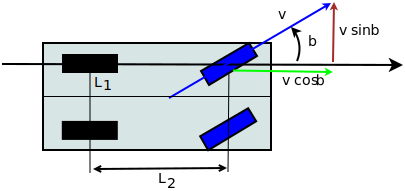
\includegraphics[width=0.6\textwidth,height=\textheight]{MotionFigures/steered.*}
\caption{Front Wheel Steered System.}
\end{figure}

\hypertarget{ackerman}{%
\subsubsection{Ackerman}\label{ackerman}}

The best known mobile vehicle design currently is the steered wheel,
specifically the Ackerman Steering design. This is our traditional car
implementation. It is a rectangular vehicle with four wheels. The front
two wheels are steered. We begin with the fixed turn angle or simple
steer model.

\[\begin{aligned}
\displaystyle
\begin{bmatrix} v \\ \dot{\theta} \end{bmatrix}
=  r \dot{\phi}
\begin{bmatrix} 1 \\ \displaystyle \frac{\sin \beta}{L_2} \end{bmatrix}
\quad \mbox{and} \quad
\begin{bmatrix} \dot{\phi}  \\ \beta \end{bmatrix}
=
\begin{bmatrix}\displaystyle  \frac{v}{r} \\ \displaystyle \sin^{-1} \frac{L_2 \dot{\theta}}{v} \end{bmatrix}
\end{aligned}\]

There are several issues with the simple design illustrated above.
During a turn the left and right wheels travel different arcs meaning
different distances, \texttt{ackermannsteeringfig}. This will cause the
wheels to skid if their rotation rates are the same. Part of the
solution is to place a differential in the axle to deliver power and
allow for different wheel speeds. The other part is to allow for
differential steering with the Ackerman design. The Ackerman steering
overcomes the issue of side slip due to the outside wheel traveling
farther than the inside wheel.

Some history here is interesting. The invention is claimed by Georg
Lankensperger (Munich) in 1817. However his agent, Rudolf Ackerman,
filed the patent and now has name credit. But, this steering system was
described 50 years earlier by Eramus Darwin (the grandfather of Charles
Darwin) in 1758 according to Desmond King-Halle in 2002 and Mr. Darwin
has claim to the invention.

\begin{quote}
To avoid skidding, the outside wheel must turn at a different angle and
rotate at a different speed than the inside wheel.
\end{quote}

To satisfy the constraint placed on by the ICR, the steering system must
satisfy the Ackerman equation:

\[\cot\theta_R - \cot\theta_L = \frac{2L_1}{L_2}\]

where \(\theta_R\) is the angle of the right wheel, \(\theta_L\) is the
angle of the left wheel, \(2L_1\) is axle length and \(L_2\) is the
wheel base length, \texttt{Fig:ackermansteerangles}. The effective
steering angle, \(\theta_S\) can be found by

\[\cot\theta_S = \frac{L_1}{L_2} + \cot\theta_R    \quad {\mbox{or} } \quad \cot\theta_S =\cot\theta_L -  \frac{L_1}{L_2}\]\[The steering angles for the Ackerman
equation.\]

The Ackerman design is one that approximates the geometric constraints
which produces the ICR. A purely mechanical solution is to embed the
geometry into the steering linkage. A triangle is formed from the
attachment points at the wheels and the center of the rear axle. By
moving the rear axle intersection, one can steer the wheels as well as
keep the zero motion lines intersecting on the rear axle. The attachment
to the wheels is called the \emph{kingpins}. The cross piece between the
Kingpins is called the \emph{tie rod}.

\begin{figure}
\centering
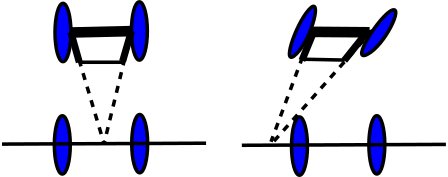
\includegraphics[width=0.6\textwidth,height=\textheight]{MotionFigures/icr-acker.*}
\caption{The Ackerman steering system.}
\end{figure}

\hypertarget{other-steered-wheel}{%
\subsubsection{Other Steered Wheel}\label{other-steered-wheel}}

As you delve into robot drive systems you begin to see that there are
many different ways that people have mounted wheels onto frames and
figured out how to steer the craft. We can only touch on a few designs
in this text and encourage the reader to look beyond this text. It can
be very entertaining to experiment with different wheel and frame
designs. Using components like Actobots
(\url{https://www.servocity.com/actobotics}), Lego, or Vex one can
quickly assemble nearly anything that your mind can dream up. One novel
approach to all wheel steering is the Syncro Drive
system~\texttt{fig:syncrodrive}. Using three or four steered wheels, the
wheels are connected by a chain or cable allowing all wheels to be
steered. Each wheel is kept in a parallel mode so that motion is
possible in any direction.

\begin{quote}
Syncro Drive System.
\end{quote}

\hypertarget{the-dubins-reeds-shepps-cars-and-other-drive-systems}{%
\subsection{The Dubins, Reeds-Shepps Cars and other drive
systems}\label{the-dubins-reeds-shepps-cars-and-other-drive-systems}}

We investigate two vehicle designs which have a similar mechanism for
steering. The first design consists of two axles with four driven
wheels. The centers of the axles are attached to the frame of the robot
using a lockable pivot. In essence, it is two differential drives
attached to a bar with the pivot mechanism (see \texttt{fig:DDD}). We
will refer to this as the Dual Differential Drive (DDD). The second
design uses four axles (or one can think of splitting the axles in the
DDD design) each with a driven wheel. The axles are attached to the body
of the robot again using locking pivots, \texttt{fig:FWS}. We will focus
on attachment points at the corners of the vehicle but other locations
such as along the center line at either end of the robot would also be
possible. For this design, mounting the pivots at the center of the axle
or at the corners of a chassis has the effect of changing the number of
pivot brakes and the costs, but does not significantly change the
kinematics. This configuration will be known as the Four Wheel Steer
(FWS). A traditional articulated steering design is shown in
\texttt{fig:AD}. The kinematics and motion curves for this design are
essentially the same as the DDD design, and as such will be treated as a
DDD steering mechanism.

\begin{quote}
Dual Differential Drive (DDD). This vehicle has single or connected axle
in the front and a single axle in the rear. The axle is connect to the
frame using a pivot which can be locked (braked) or free.

Four Wheel Steer (FWS). This vehicle has four axles each is connected to
the frame by a lockable pivot. In addition to motion see in the DDD
design, if there is sufficient rotational motion in the axles, this
conifguration can spin in place.

Articulated Drive (AD). This is a common design in heavy equipment like
articulated front loaders. The motion is similar to that found in the
DDD design and can be driven with an unlocked pivot (brake not
required).
\end{quote}

When a wheel motor is activated, it will cause the axle to rotate about
the pivot. Once the desired angle is achieved, the pivot is locked
leaving the wheels in the steered configuration. The pivot joints are
binary in the sense that they are completely locked or completely free.
This is done by a normally closed brake attached to the pivots and will
allow free motion when power is applied to the pivot brake. When power
is interrupted, the pivot brake locks down. Expected initial operation
of the test unit is to alternate between a fixed position while aligning
wheels and vehicle motion with the pivot brakes locked.

In terms of movement in the plane, the solid axle system is a dual
differential drive. For the purposes of understanding motion curves we
can view it as a two wheel (bicycle) design. Since we use four drive
motors there is no need for a differential. The FWS axle mounted on the
box can emulate Ackerman steering and does not suffer from wheel slip or
slide. We will see that this design has greater maneuverability in
comparison to a double Ackerman steered vehicle. In either case, we have
two situations with a moving vehicle: driving straight paths and
circular paths. Not found in Ackerman systems, the FWS design can
additionally rotate in place if the axle is allowed to rotate out
\(45^\circ\) or more.

\begin{quote}
The forward motion curves. Left: traditional Dubins Car. Right: forward
motion of the DDD vehicle.
\end{quote}

For the DDD design, using the bicycle approximation, the radius of
curvature is given as a function of the maximum axle rotation and the
wheelbase. Let the axle turn angle be \(\theta\) and the wheel base
given by \(d\), then the radius of curvature is given by

\[r  = d/(2\sin\theta)\]

\texttt{fig:turngeo} (left). In addition, the DDD can move linearly in
directions angled off the forward direction of the vehicle if the axles
are parallel and have nonzero axis angle in reference to the forward
vehicle normal \texttt{fig:fmotion}. The direction off of the forward
normal direction is given by the axle angles and if the front and rear
axles are not parallel, then a circular path will occur with direction
off of the forward direction as seen with parallel axles.

\begin{quote}
Turn geometry for the DDD (left) and FWS (right) designs.
\end{quote}

The FWS design can adjust to the radius of curvature for both inside and
outside wheels. The radius of curvature for the vehicle center is the
average of the inside and outside circle radii:

\[\overline{r} = (r_1+r_2)/2 = d\left(1/(4\sin\theta_1) + 1/(4\sin\theta_2)\right)\]

\texttt{fig:turngeo}. For this design, we have the ability to move as
with the DDD and in addition rotate in place. Both systems can also move
forwards and reverse. Thus orientation and direction may be changed at
any point along the trajectory.

For the DDD, there are four motors (with associated electronics) and two
pivot brakes (and associated electronics). The FWS design adds two pivot
brakes in addition to the DDD cost. The operating assumption here is
that mechanical holding torque can be gained more cheaply than
electrical turning torque. The term ``cheap'' will refer to dollar cost
or to electrical power depending on the context. The dollar cost range
for motors, motor drivers, electromagnetic brakes, etc., varies greatly.
In our application, we found the prices to be fairly close between
brakes and motors but the prices for driving electronics was
significantly cheaper for the brakes as they operate like solenoids and
the more complicated motor driver hardware was not required.

We have found that we don't need a brake for the DDD system which
removes both financial and electrical costs associated with the
eliminated systems. For the FWS system, we can purchase a normally
locked brake. Power is applied only when adjustments are required thus
removing the need for holding current.
